\documentclass[12pt,a4paper]{article}
\usepackage{better_poster}
\usepackage{enumitem}

% ---- fill in from here

% authors
\title{Quantificare l’effetto di interesse}
\author{Zandonella Callegher* C., Toffalini E., \& Altoè G.\\
\scriptsize *claudio.zandonellacallegher@phd.unipd.it}

% type of poster: [exp]erimental results, [methods], [theory]
% Disclaimer: the original classification had "study" and "intervention" as separate categories. I group them under experimental results.
\newcommand\postertype{exp} % [exp],[methods],[theory]

\begin{document}

% main point of your study
\makefinding{
\textbf{L'Elicitazione} permette di utilizzare la \textbf{conoscenza degli esperti} nelle proprie analisi.
}


% \makemain{
% }{

% }


% the main text of your poster goes here
\makemain{
\vspace{2em}

Quantificare l'\textbf{effetto di interesse} è necessario sia per compiere una \textbf{power-analysis}, sia per formalizzare le proprie \textbf{ipotesi di ricerca}.


\section*{Elicitazione degli esperti}

\begin{itemize}[leftmargin=*]
    \item{Quando precedenti studi sono limitati, le indicazioni degli esperti sono un'utile risorsa.} 
    \item{L'elicitazione permette di definire una distribuzione di probabilità che rappresenti propriamente la conoscenza e l'incertezza degli esperti.}
\end{itemize}

\centering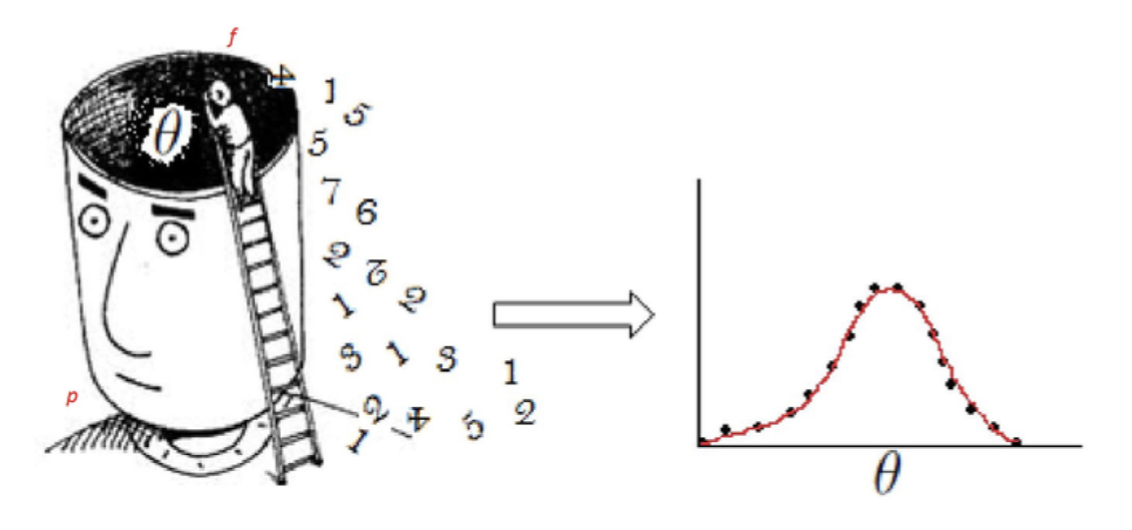
\includegraphics[width=.95\linewidth]{images/elicitation}
\begin{center}\tiny Immagine da Barrera-Causil et al. (2019)\end{center}
\vfill
}
% If you have extra figures or data to show
\makeextracolumn{
    \centering
    \textit{Chi sono più alti i ragazzi o le ragazze?}
    \vspace{1em}
    
    \scriptsize Immaginate vengano formate 10 coppie, ognuna composta da un ragazzo e una ragazza della stessa età scelti casualmente. In quante delle 10 coppie il ragazzo sarà più alto della ragazza?
    \vfill
    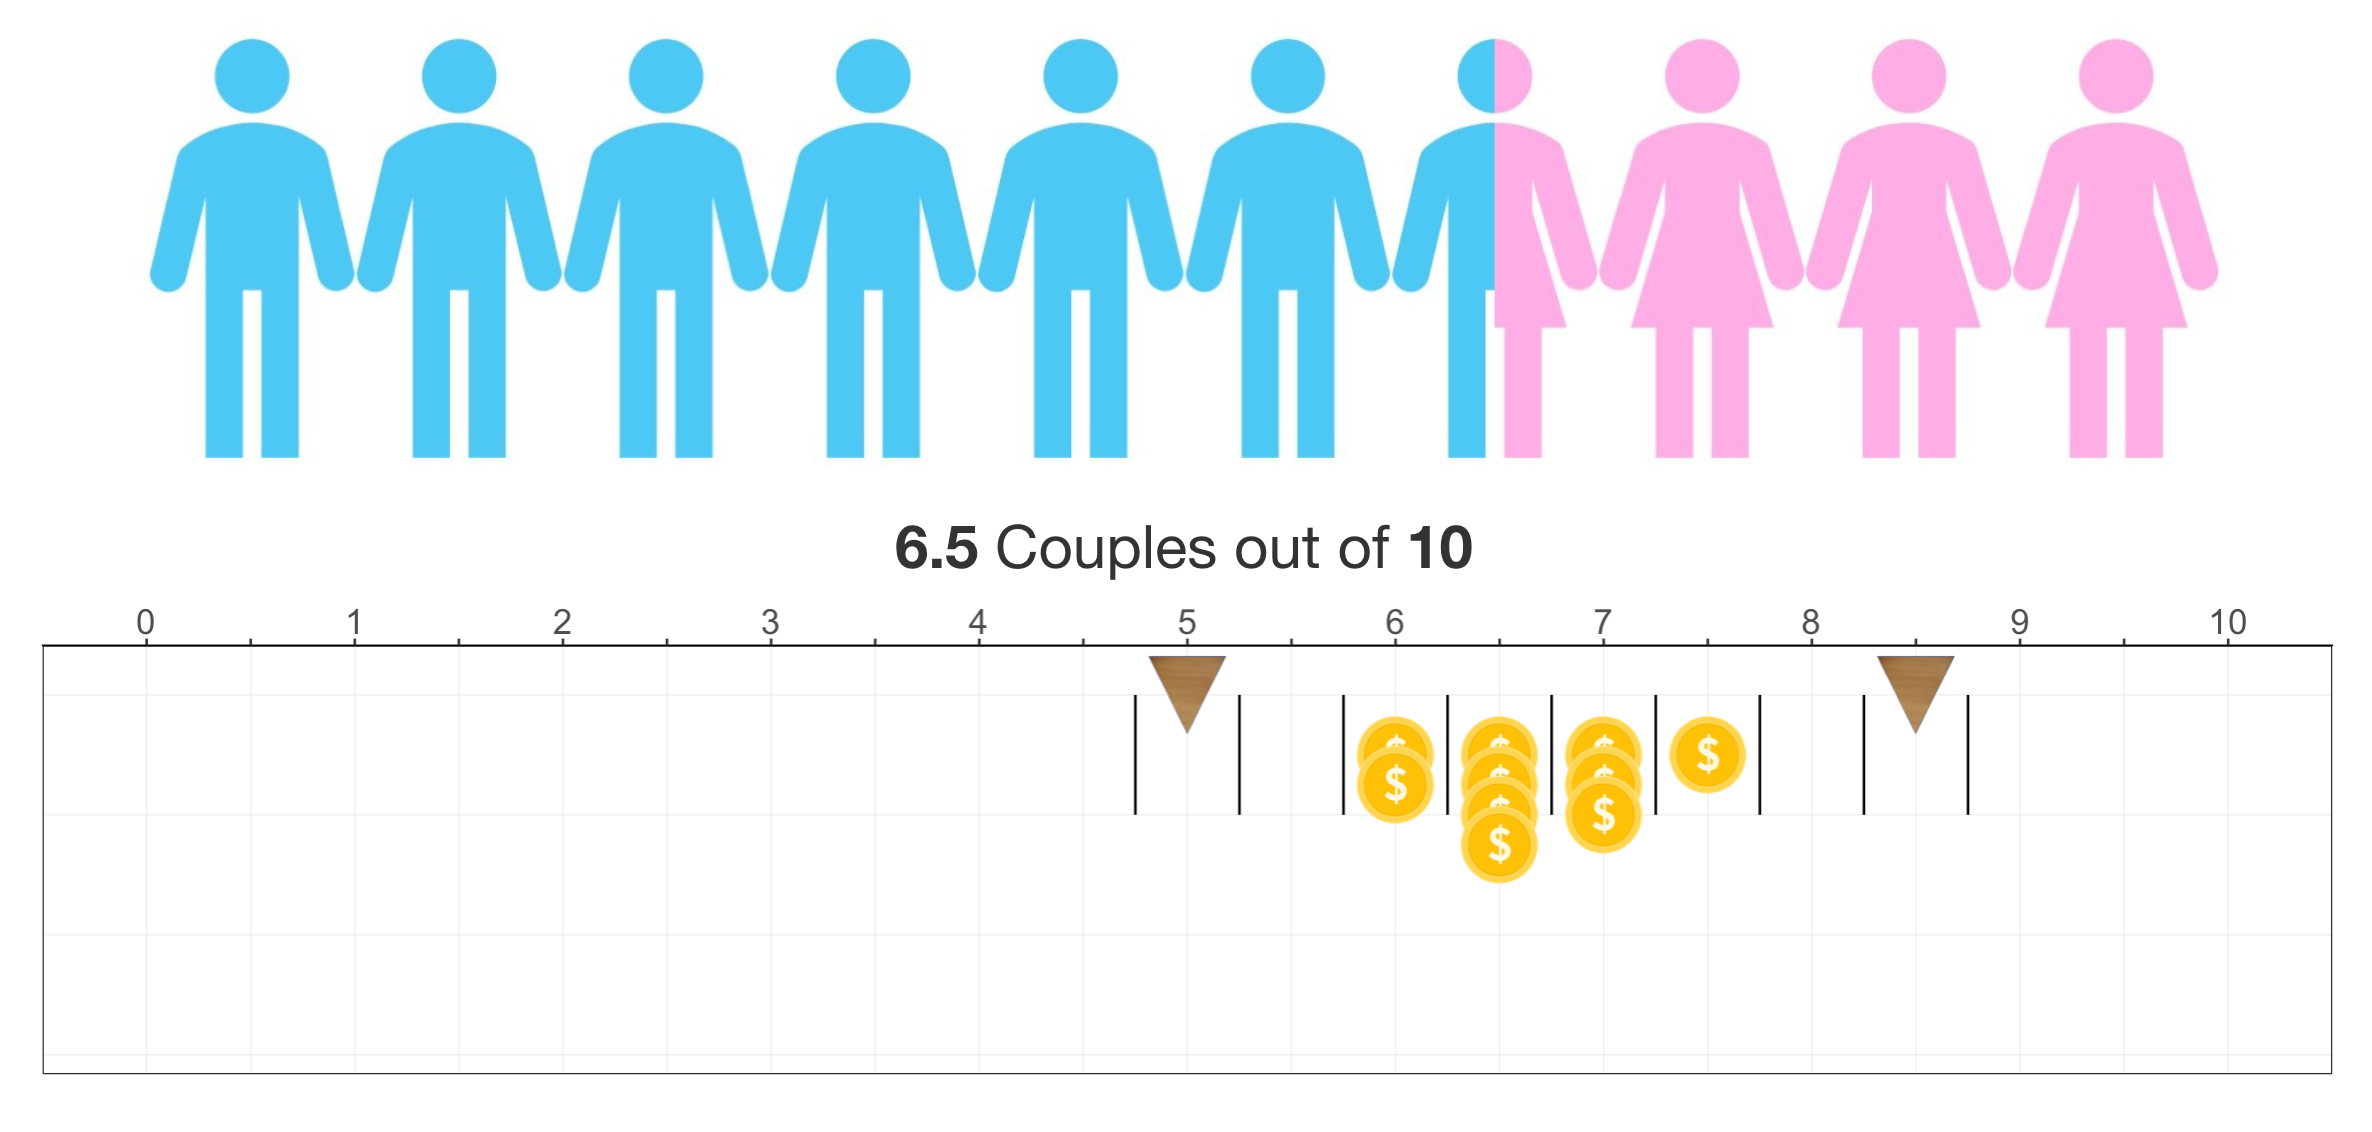
\includegraphics[width=0.9\linewidth]{images/app2}
    \vfill
    12 anni ($d=-0.31$)
    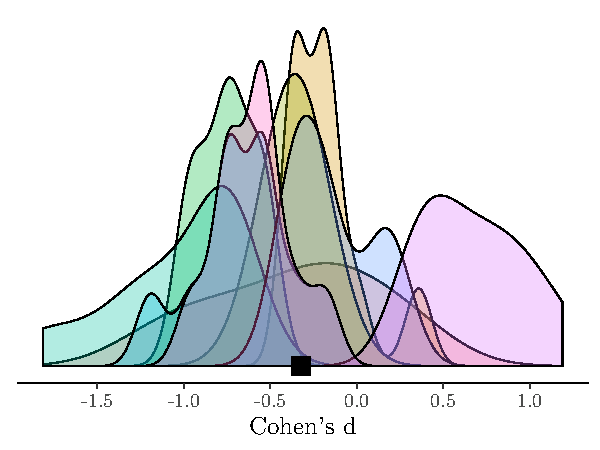
\includegraphics[width=0.5\linewidth]{images/age_12_mixed-1}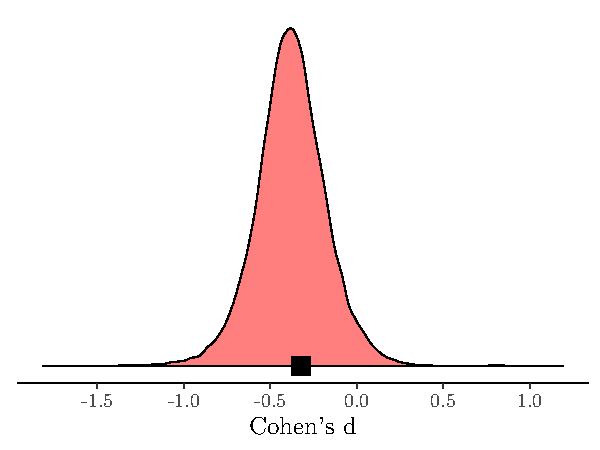
\includegraphics[width=0.5\linewidth]{images/age_12_model-1}
    \vfill
    14 anni ($d=0.46$)
    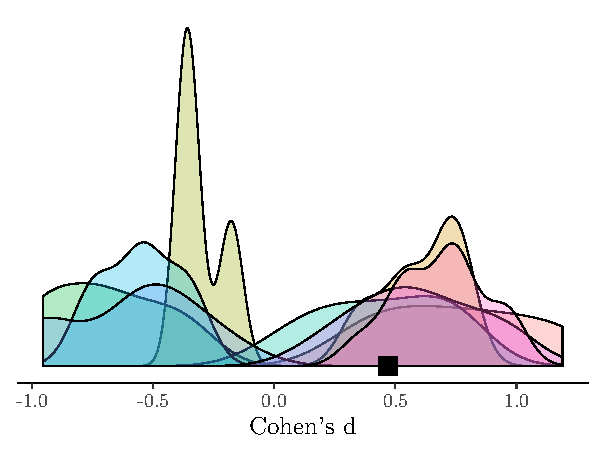
\includegraphics[width=0.5\linewidth]{images/age_14_mixed-1}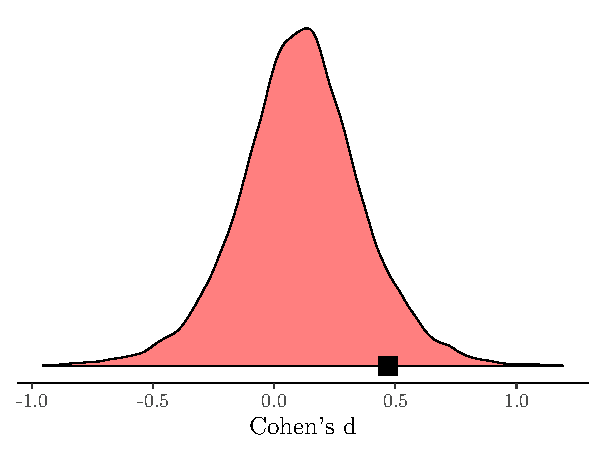
\includegraphics[width=0.5\linewidth]{images/age_14_model-1}
    \vfill
    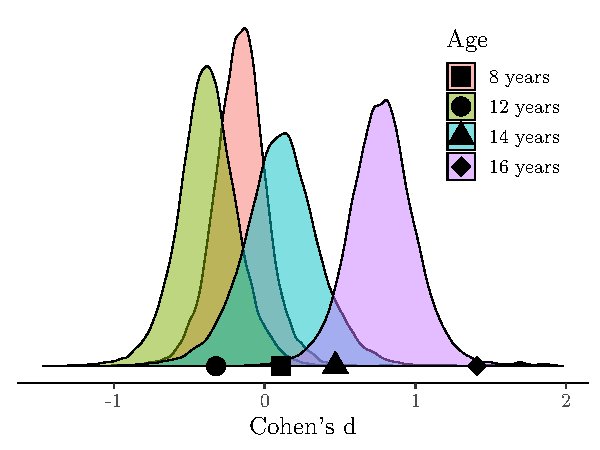
\includegraphics[width=0.9\linewidth]{images/final-1}
    \vfill
    
    
}

% footer
% generate qr code from https://www.qr-code-generator.com/ and replace qr_code.png
% default: barcode on the left

    \vspace*{\fill}
    \noindent\makebox[\linewidth][c]{%
      \colorbox{\postertype}{%
        \parbox[c][0.11\paperheight][c]{\paperwidth}{%
          \hspace*{\dimexpr\hoffset+\oddsidemargin+1in\relax}%
          \begin{centering}
              \begin{minipage}[c][0.10\paperheight][c]{0.15\textwidth}
                    \centering
\includegraphics[height=0.05\paperheight]{images/LaTeX_logo2}
              \end{minipage}
              \hfill
              \begin{minipage}[c][0.12\paperheight][c]{0.15\textwidth}
                    \centering
\includegraphics[height=0.06\paperheight]{images/R_logo.png}
              \end{minipage}
              \hfill
              \begin{minipage}[c][0.12\paperheight][c]{0.15\textwidth}
                    \centering
\includegraphics[height=0.10\paperheight]{images/Download_poster}
              \end{minipage}
              \hfill
              \begin{minipage}[c][0.12\paperheight][c]{0.15\textwidth}
                    \centering
\includegraphics[height=0.08\paperheight]{images/Psicostat_circle}
              \end{minipage}
              \hfill
              \begin{minipage}[c][0.12\paperheight][c]{0.15\textwidth}
                    \centering
\includegraphics[height=0.08\paperheight]{images/unipd_logo_uff.png}
              \end{minipage}
              \hfill
          \end{centering}
        }%
      }%
    }\par\medskip

% replace with this like for barcode on the right
%\makealtfooter{images/uni_logo.png}{images/qr-code.png}

\end{document}